\chapter{Przykładowe aplikacje}
\label{cha:przyklady}

W niniejszym rozdziale pracy zaprezentowano przykładowe aplikacje zaimplementowane w języku Erlang i uruchomione na maszynie wirtualnej opisywanej w pracy. Platformą, na której uruchamiane były przykłady był mikrokontroler LPC1769 z procesorem ARM Cortex-M3 pod kontrolą mikrojądra FreeRTOS.

Wszystkie aplikacje zostały skompilowane przy użyciu narzędzia opisanego w dodatku \ref{cha:builder}. Kody źródłowe aplikacji zostały umieszczone na płycie CD dołączonej do pracy.

\section{Silnia}
\label{sec:przykladySilnia}

\subsection{Cel aplikacji}

Aplikacja miała na celu uruchomienie przykładowego sekwencyjnego programu zaimplementowanego w języku Erlang w dwóch wersjach: z rekurencją ogonową oraz bez tego typu rekurencji.

Rekurencja ogonowa charakteryzuje się tym, że wynik wywołania funkcji rekurencyjnej całkowicie zależy od wyniku rekurencyjnego wywołania funkcji.
Nie ma zatem konieczności powrotu do poprzedniego wywołania funkcji w celu ustalenia aktualnej wartości funkcji, a co za tym idzie zapisywania na stosie adresu powrotu i wyrażeń potrzebnych do wyliczenia zwracanego wyniku.
Kompilator Erlanga automatycznie wykrywa funkcje ogonowo-rekurencyjne i optymalizuje kod pośredni pod kątem użytego rozmiaru stosu (por. np. opis instrukcji \texttt{call} i \texttt{call\_only} na liście instrukcji kodu pośredniego na str. \pageref{sec:opsOps}).

Listingi \ref{lis:fac_facERL} oraz \ref{lis:fac_fac2ERL} przedstawiają kody źródłowe dwóch funkcjonalnie równoważnych sobie funkcji (\texttt{fac/1}) obliczających silnię liczby naturalnej.

\begin{figure}
\begin{multicols}{2}
\begin{lstlisting}[style=erlang, caption=Kod modułu \texttt{fac.erl}, label=lis:fac_facERL]
-module(fac).

-export([fac/1]).

fac(0) ->
    1;
fac(N) ->
    N*fac(N-1).



\end{lstlisting}

\columnbreak

\begin{lstlisting}[style=erlang, caption=Kod modułu \texttt{fac2.erl}, label=lis:fac_fac2ERL]
-module(fac2).

-export([fac/1]).

fac(N) ->
    fac(N, 1).

fac(0, Acc) ->
    Acc;
fac(N, Acc) ->
    fac(N-1, N*Acc).
\end{lstlisting}
\end{multicols}
\end{figure}

Funkcja z modułu \texttt{fac} wykorzystuje do tego celu tradycyjną rekurencję, uzależniając wynik zwrócony przez funkcję nie tylko od rekurencyjnego wywołania samej siebie, ale także od argumentu z jakim została wywołana. 

Funkcja zaimplementowana w module \texttt{fac2} wykorzystuje dodatkowy argument, tzw. akumulator, którego aktualna wartość przekazywana jest wraz z każdym kolejnym wywołaniem, a na samym końcu zwracana.
Dzięki zastosowaniu tego podejścia funkcja ta jest ogonowo-rekurencyjna, co pozwala na optymalizację użycia stosu przez kompilator Erlanga w kodzie pośrednim.

Celem eksperymentu było uruchomienie dwóch ww. funkcji obliczających silnię dla różnych wejściowych liczb naturalnych od 1 do 200. Pozwoliło to na sprawdzenie działania podstawowych elementów maszyny wirtualnej, m.in. interpretera kodu pośredniego, \emph{garbage collectora} czy arytmetyki dużych liczb (do zapisania wyniku $200!$ potrzebnych jest 156 bajtów).


\subsection{Uzyskane wyniki}

Silnia została obliczona dla wejściowych liczb: 1, 11 (wynik $11!$ jest ostatnim, jaki mieści się na 28 bitach i może zostać przechowany jako wyrażenie typu \textbf{SMALL}), 12 (wynik $12!$ jest ostatnim, jaki mieści się na 32 bitach i jest zarazem pierwszym, który do przechowania potrzebuje typu danych \textbf{BIGNUM}), 25, 50, 75, 100, 125, 150, 175 i 200. Dla wszystkich wartości wejściowych, dla obu modułów, uzyskano poprawne wartości silni.

Obliczenia zostały wykonane w kontekście procesu Erlanga, który był jedynym uruchomionym w~tym momencie na maszynie wirtualnej.

Czas wykonania mierzony był przy użyciu sprzętowego licznika wbudowanego w mikrokontroler, taktowanego zegarem o częstotliwości 1 MHz.

Rezultaty uzyskane w trakcie uruchomień zostały zaprezentowane na rysunku \ref{fig:facGraphs}.


Zgodnie z oczekiwaniami rozmiar sterty procesu w przypadku modułu \texttt{fac} rósł znacznie szybciej niż w przypadku modułu \texttt{fac2}, osiągając aż 610 słów maszynowych
w porównaniu do 90 słów w~przypadku funkcji ogonowo-rekurencyjnej dla obliczenia wyniku $200!$.
Na samo przechowanie stosu wywołań w pierwszym przypadku konieczne jest 400 słów maszynowych (200 liczb \textbf{SMALL} i 200 adresów powrotu).

Dużo większy rozmiar sterty dla pierwszego z modułów miał bezpośredni wpływ na dużo rzadsze uruchomienia \emph{garbage collectora}.
Ponieważ wyrażenia zajmujące znaczną część sterty (duże liczby) potrzebne były tylko w czasie jednego rekurencyjnego wywołania funkcji, przy każdym jego uruchomieniu zwalniana byłą dużą część pamięci. Większa część zaalokowanej sterty mogła zostać zatem później wykorzystana przez kolejne wywołania funkcji.

Z tego samego powodu w przypadku funkcji ogonowo-rekurencyjnej, \emph{garbage collectorowi} udało zwolnić się większą część pamięci (ok. 4500 słów maszynowych w porównaniu do ok. 3500 słów maszynowych).

Sam czas wykonywania kodu był nieco większy w przypadku modułu \texttt{fac} (2981 \textmugreek s w porównaniu do 2108 \textmugreek s), co wynika bezpośrednio z większej liczby instrukcji w kodzie pośrednim.
Czas spędzony na odśmiecaniu sterty procesu (ok. 43\% łącznego czasu wykonania programu w przypadku modułu \texttt{fac2} w porównaniu do ok. 21\% czasu dla drugiego modułu) miał jednak decydujący wpływ na łączny czas obliczenia silni, który okazał się wyraźnie większy dla modułu z funkcją ogonowo-rekurencyjną (4920 \textmugreek s w porównaniu do 3750 \textmugreek s).

Dla porównania, obie powyższe funkcje obliczające silnię z 200 na maszynie wirtualnej BEAM na komputerze z systemem operacyjnym MacOS X i procesorem Intel Core i7, wykonały się w ok. 1800 \textmugreek s.
Należy wspomnieć, że początkowy rozmiar sterty procesu został ustawiony na 12 słów maszynowych, tak jak jest to w przypadku maszyny implementowanej w pracy.


Różnicę można również zauważyć w liczbie wykonanych redukcji przez procesy, która jest nieco większa w przypadku wykonywania kodu z modułu \texttt{fac}.
Powodem tego jest fakt, że w całkowitą liczbę redukcji procesu wliczany jest czas uruchomienia \emph{garbage collectora}, ale tylko w przypadku gdy jest on uruchamiany przez instrukcje z rodziny \texttt{allocate} (opkody 12-15). Jeżeli \emph{garbage collector} uruchomiony zostanie w trakcie operacji arytmetycznej, redukcje nie są doliczane.
Ponieważ kod modułu \texttt{fac2} nie używa stosu, liczba redukcji przez niego wykonana pochodzi tylko i wyłącznie z wywołań funkcji.

\begin{figure}

\begin{multicols}{2}

\begin{gnuplot}[terminal=epslatex,terminaloptions=color,scale=0.7]
	set grid
	set title 'Pamięć zwolniona przez \emph{garbage collector}'
	set ylabel 'słowa maszynowe'
	set xlabel '$n$'
	set yr [0:5000]
	set size ratio 0.8
	plot 'facstats.csv' using 1:2 w p pt 7 ps 1 title 'fac:fac($n$)',\
			'facstats.csv' using 1:2 smooth csplines lt 3 lw 4 lc 1 notitle,\
			'fac2stats.csv' using 1:2 w p pt 7 ps 1 lc 3 title 'fac2:fac($n$)', \
			'fac2stats.csv' using 1:2 smooth csplines lt 3 lw 4 lc 3 notitle
\end{gnuplot}

\begin{gnuplot}[terminal=epslatex,terminaloptions=color,scale=0.7]
	set grid
	set title 'Uruchomienia \emph{garbage collectora}'
	set ylabel 'uruchomienia'
	set xlabel '$n$'
	set yr [0:180]
	set size ratio 0.8
	plot 'facstats.csv' using 1:3 w p pt 7 ps 1 title 'fac:fac($n$)',\
			'facstats.csv' using 1:3 smooth csplines lt 3 lw 4 lc 1 notitle,\
			'fac2stats.csv' using 1:3 w p pt 7 ps 1 lc 3 title 'fac:fac2($n$)', \
			'fac2stats.csv' using 1:3 smooth csplines lt 3 lw 4 lc 3 notitle
\end{gnuplot}

\begin{gnuplot}[terminal=epslatex,terminaloptions=color,scale=0.7]
	set grid
	set title 'Czas działania'
	set ylabel 'czas ($\mu s$)'
	set xlabel '$n$'
	set size ratio 0.8
	plot 'facstats.csv' using 1:5 w p pt 7 ps 1 title 'całkowity fac:fac($n$)',\
			'facstats.csv' using 1:5 smooth csplines lt 3 lw 4 lc 1 notitle,\
			'fac2stats.csv' using 1:5 w p pt 7 ps 1 lc 3 title 'całkowity fac:fac2($n$)', \
			'fac2stats.csv' using 1:5 smooth csplines lt 3 lw 4 lc 3 notitle,\
\end{gnuplot}


\begin{gnuplot}[terminal=epslatex,terminaloptions=color,scale=0.7]
	set grid
	set title 'Wykonane redukcje'
	set ylabel 'redukcje'
	set xlabel '$n$'
	set size ratio 0.8
	plot 'facstats.csv' using 1:4 w p pt 7 ps 1 title 'fac:fac($n$)',\
			'facstats.csv' using 1:4 smooth csplines lt 3 lw 4 lc 1 notitle,\
			'fac2stats.csv' using 1:4 w p pt 7 ps 1 lc 3 title 'fac:fac2($n$)', \
			'fac2stats.csv' using 1:4 smooth csplines lt 3 lw 4 lc 3 notitle
\end{gnuplot}


\begin{gnuplot}[terminal=epslatex,terminaloptions=color,scale=0.7]
	set grid
	set title 'Rozmiar sterty procesu'
	set ylabel 'słowa maszynowe'
	set xlabel '$n$'
	set size ratio 0.8
	plot 'facstats.csv' using 1:9 w p pt 7 ps 1 title 'fac:fac($n$)',\
			'facstats.csv' using 1:9 w steps lt 3 lw 4 lc 1 notitle,\
			'fac2stats.csv' using 1:9 w p pt 7 ps 1 lc 3 title 'fac:fac2($n$)', \
			'fac2stats.csv' using 1:9 w steps lt 3 lw 4 lc 3 notitle,\
\end{gnuplot}

\begin{gnuplot}[terminal=epslatex,terminaloptions=color,scale=0.7]
	set grid
	set title 'Czas działania'
	set ylabel 'czas ($\mu s$)'
	set xlabel '$n$'
	set yr [0:4000]
	set size ratio 0.8
	plot 'facstats.csv' using 1:7 w p pt 7 ps 1 title 'kod fac:fac($n$)',\
			'facstats.csv' using 1:7 smooth csplines lt 3 lw 4 lc 1 notitle,\
			'fac2stats.csv' using 1:7 w p pt 7 ps 1 lc 3 title 'kod fac:fac2($n$)', \
			'fac2stats.csv' using 1:7 smooth csplines lt 3 lw 4 lc 3 notitle,\
			'facstats.csv' using 1:6 w p pt 5 ps 1 lc 1 title 'GC fac:fac($n$)',\
			'facstats.csv' using 1:6 smooth csplines lt 3 lw 4 lc 1 notitle,\
			'fac2stats.csv' using 1:6 w p pt 5 ps 1 lc 3 title 'GC fac:fac2($n$)', \
			'fac2stats.csv' using 1:6 smooth csplines lt 3 lw 4 lc 3 notitle
\end{gnuplot}

\end{multicols}

\caption{Porównanie wyników uruchomienia modułów \texttt{fac} oraz \texttt{fac2} na implementowanej maszynie wirtualnej.}
\label{fig:facGraphs}

\end{figure}

\subsection{Wnioski}

Eksperymentalne uruchomienia funkcji obliczających silnię zwróciły poprawne wyniki, testując w~ten sposób arymetykę dużych liczb zaimplementowaną w maszynie wirtualnej.
Zmierzone czasy wykonania zarówno kodu jak i odśmiecania mogą stanowić punkt odniesienia przy przewidywania narzutu, jaki do aplikacji uruchamianej na mikrokontrolerze może wprowadzić maszyna wirtualna.
Na ich podstawie można wyciągnąć wniosek, że rekurencja ogonowa co prawda wykorzystuje zdecydowanie mniej pamięci, jednak przez dużą liczbę odśmieceń zajmuje więcej czasu. 

W momencie projektowania funkcji w Erlangu, która uruchamiana będzie na szybkim procesorze i~przy dostępnej dużej ilości pamięci, wybór pomiędzy rekurencją ogonową a tradycyjną nie ma większego znaczenia (o ile liczba wywołań nie jest bardzo duża, mogąca spowodować skończenie się dostępnej pamięci) i wybór implementacji powinien zostać podyktowany czytelnością kodu funkcji. Jednak w przypadku urządzeń wbudowanych, ze względu na bardzo ograniczone rozmiary zasobów, zawsze powinna być wybierana rekurencja ogonowa, która po optymalizacji kompilatora nie będzie używać stosu procesu w momencie rekurencyjnych wywołań funkcji.
Wydajność konkretnej aplikacji, poprzez zmniejszenie liczby uruchomień \emph{garbage collectora}, może zostać poprawiona przez wybór w pliku konfiguracyjnym początkowego rozmiaru sterty procesu, adekwatnego do jego logiki.


\section{Kontrola diod LED przez procesy}
\label{sec:przykladyDiody}

\subsection{Cel aplikacji}

Celem aplikacji było uruchomienie przykładowego programu korzystającego ze współbieżnych cech języka Erlang.
Aplikacja miała pozwolić na sprawdzenie działania takich funkcjonalności maszyny wirtualnej jak:
przesyłania i odbierania wiadomości między procesami, propagacji zakończenia działania procesu (\emph{link}) czy mechanizmów zarządzania czasem (przeterminowania i wysyłania wiadomości do innych procesów z opóźnieniem).

W tym celu zaimplementowano dwa moduły: \texttt{led\_sup} i \texttt{led\_drv}, których zadaniem była kontrola diod LED, przez zaimplementowane funkcje kontrolujące GPIO, w dwóch kolorach: czerwonym i~zielonym.
W systemie uruchomiony był jeden proces implementujący logikę pierwszego z modułów oraz osiem procesów - drugiego z nich.
Każdy z procesów \texttt{led\_drv} kontrolował stan jednej zielonej diody - zapalał lub gasił ją po otrzymaniu wiadomości z procesu \texttt{led\_sup}. Proces ten, w odstępie sekundowym, wysyłał do trzech losowych procesów wiadomość o zmianie stanu diody. Dodatkowo, w logice procesu ustawione zostało przeterminowanie, efektem którego było zakończenie się działania procesu w~sytuacji, gdy żadna wiadomość kontrolująca stan diody nie przyszła do skrzynki odbiorczej procesu w~odstępie 2 sekund.

Stan systemu wizualizowało dodatkowo osiem czerwonych diod, które były zgaszone w momencie gdy procesy kontrolujące odpowiadający im diody zielony były uruchomione i zapalone w przeciwnym wypadku.
Pojedynczy proces był procesem nadzorczym (\emph{supervisor}), którego zadaniem było ponowne uruchamianie kończących się procesów kontrolujących diody zielone. W tym celu, proces ten musiał działać jako proces przechwytujący wyjścia procesów z nim powiązanych jako wiadomości (co w języku Erlang realizowane jest poprzez ustawienie flagi procesu \texttt{trap\_exit} na \texttt{true}).
Dla czytelniejszej prezentacji stanu systemu w przykładzie, proces kontrolujący diodę zieloną restartowany był dopiero po upływie przynajmniej dwóch sekund po otrzymaniu wiadomości o zakończeniu się jego poprzednika.

Zależności między procesami uruchomionymi w ramach przykładowej aplikacji zostały zaprezentowane na rysunku \ref{fig:exampleledprocesses}. Fizyczna realizacja podłączeń diod, sterowanych stanem niskim, do mikrokontrolera wykorzystanego w przykładzie przedstawiona została na rysunku \ref{fig:exampleled}. Na obu rysunkach diody zostały oznaczone tymi samymi symbolami.

\begin{figure}[h]
\centerline{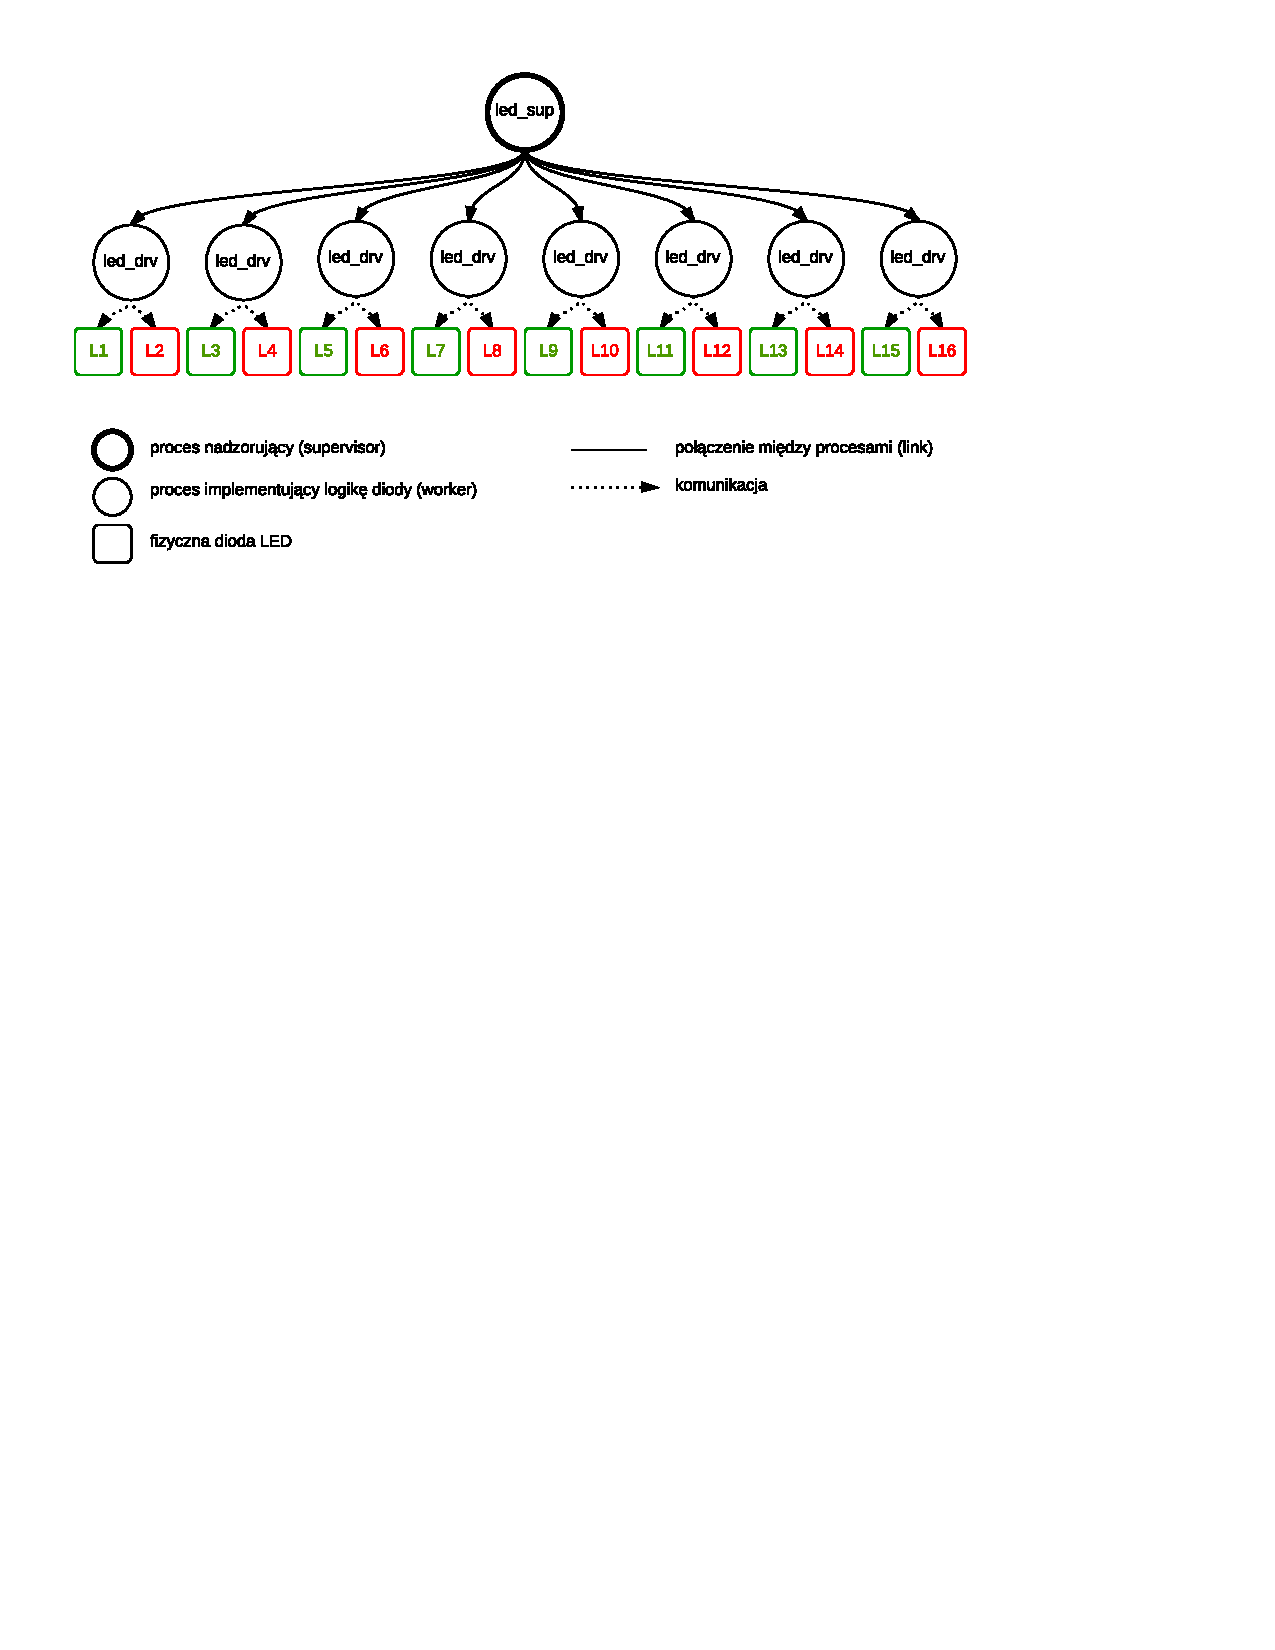
\includegraphics[scale=1, clip, trim=10mm 175mm 135mm 10mm]{example_led_processes}}
\caption{Struktura procesów w aplikacji i kontrolowanych przez nie diod}
\label{fig:exampleledprocesses}
\end{figure}

\begin{figure}[h]
\centerline{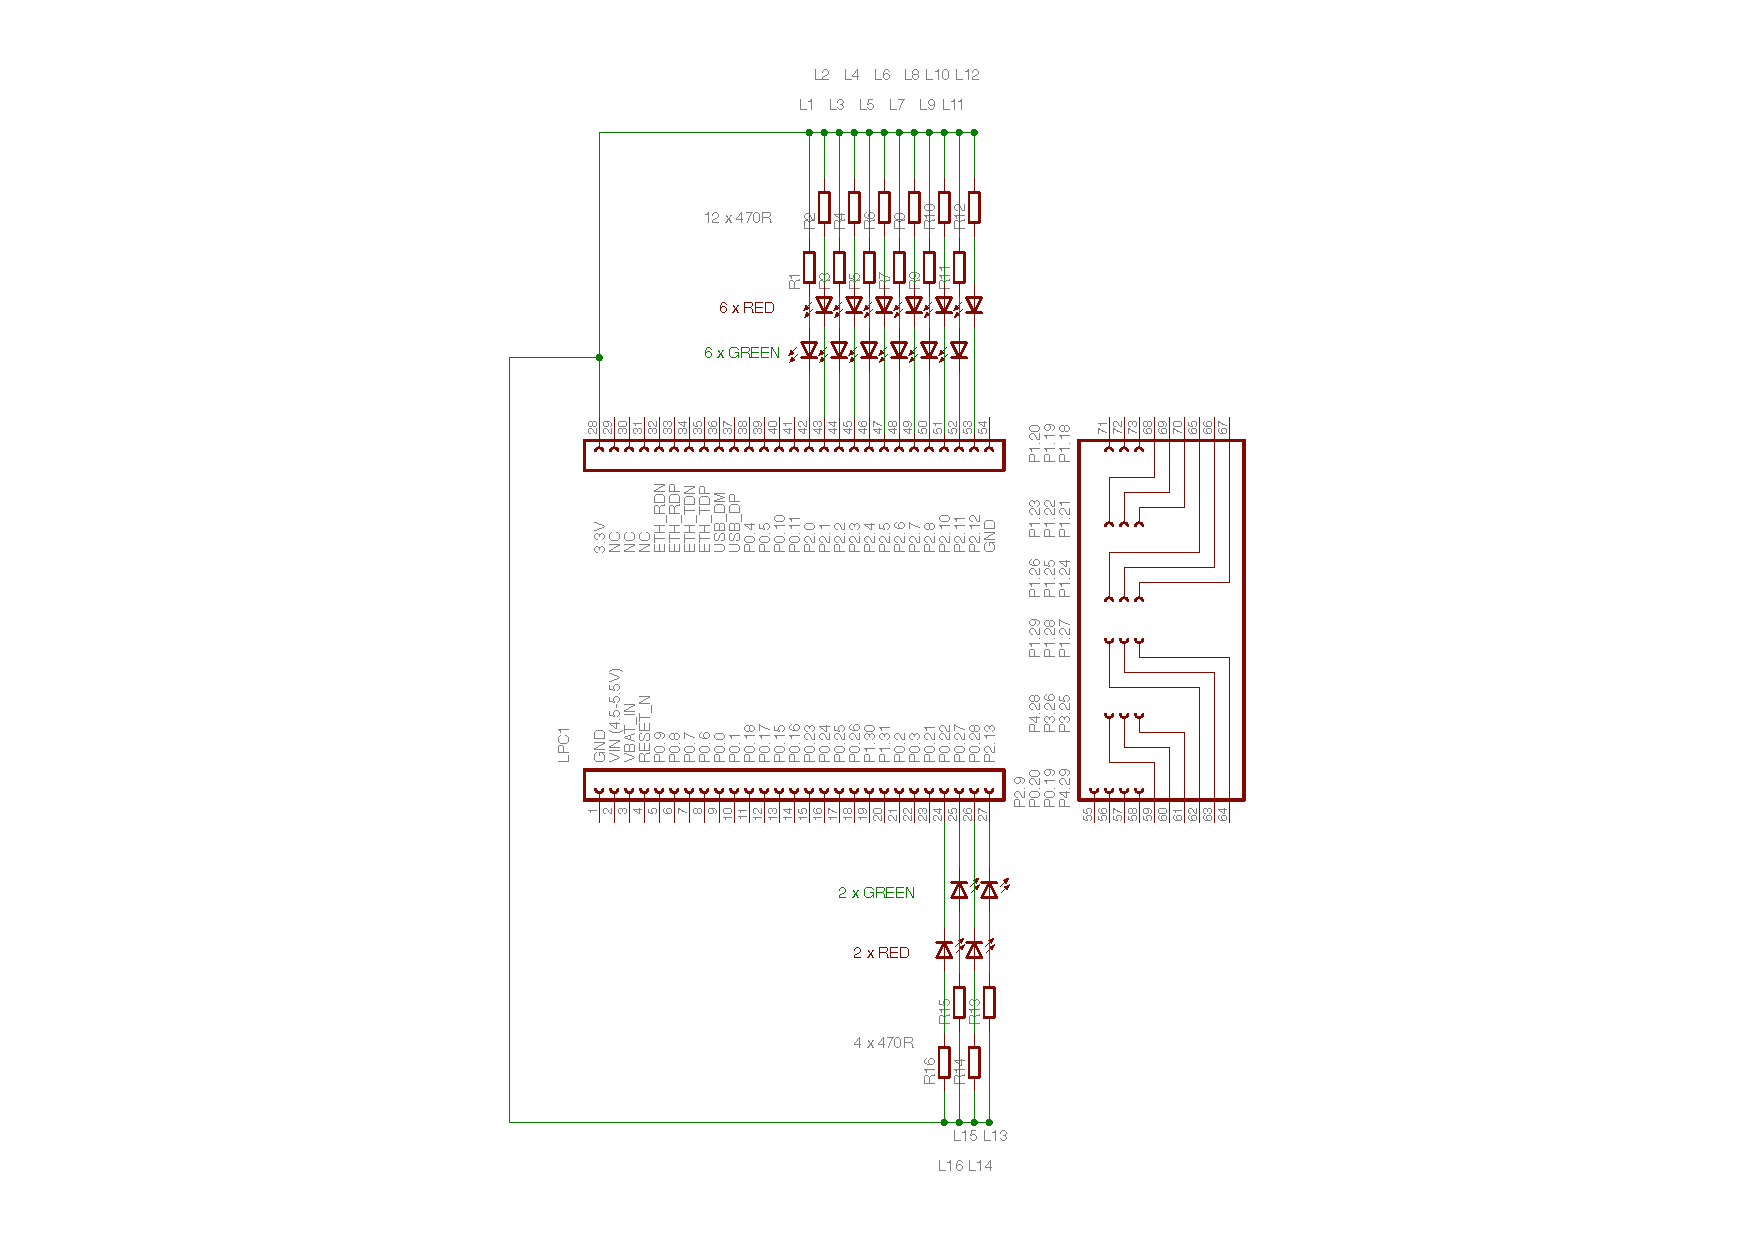
\includegraphics[scale=1, clip, trim=0mm 40mm 0mm 35mm]{example_led}}
\caption{Schemat podłączenia diod LED do płytki prototypowej z mikrokontrolerem LPC1769}
\label{fig:exampleled}
\end{figure}


\subsection{Uzyskane wyniki}

\subsection{Wnioski}


\section{Sterownik RFM73}
\label{sec:przykladyRfm}

\subsection{Cel aplikacji}

Celem aplikacji było zaimplementowanie biblioteki sterownika do modułu radiowego RFM73 \cite{RFM73}, produkowanego przez firmę Hope Microelectronics.
Ten tani układ (koszt jednej sztuki to ok. 10 PLN) pozwala na komunikację bezprzewodową w paśmie 2,4 GHz z szybkością dochodzącą do 2 Mbps. Warstwa sprzętowa zapewnia możliwość wysłania pakietu składającego się z maksymalnie 32 bajtów.
Odpowiedzialność za implementację protokołu pozwalającego na wysyłanie dłuższych pakietów należy już jednak do programisty.

Moduł komunikuje się ze światem zewnętrznym dzięki wbudowanemu w niego mikrokontrolerowi, za pomocą interfejsu szeregowego SPI (\emph{Serial Peripheral Interface}). Sam układ zapewnia także sprawdzanie poprawności pakietu za pomocą sumy kontrolnej, prosty mechanizm retransmisji czy adresowania urządzeń w sieci.

Typowymi zastosowaniami modułu mogą być takie urządzenia jak np:
\begin{itemize}
\item urządzenia zdalnego sterowania;
\item sensory przesyłające dane pomiarowe;
\item urządzenia peryferyjne do komputerów osobistych.
\end{itemize}

Implementowana aplikacja miała pozwolić na przykładowe obsłużenie urządzenia peryferyjnego w~języku Erlang, w tym wypadku za pomocą zaimplementowanych funkcji wbudowanych obsługujących interfejs SPI.
Udostępnione funkcje wyprowadzeń z modułu RFM73 pozwoliły również na zaimplementowanie biblioteki w ten sposób, by możliwe było przetestowanie tłumaczenia przerwań zewnętrznych zgłaszanych do mikrokontrolera na wiadomości wysyłane do procesów.

Fizyczna realizacja podłączeń układu do płytki uruchomieniowej z mikrokontrolerem LPC1769, na którym uruchamiany był niniejszy przykład została zaprezentowana na rysunku \ref{fig:examplerfm}.

\begin{figure}[h]
\centerline{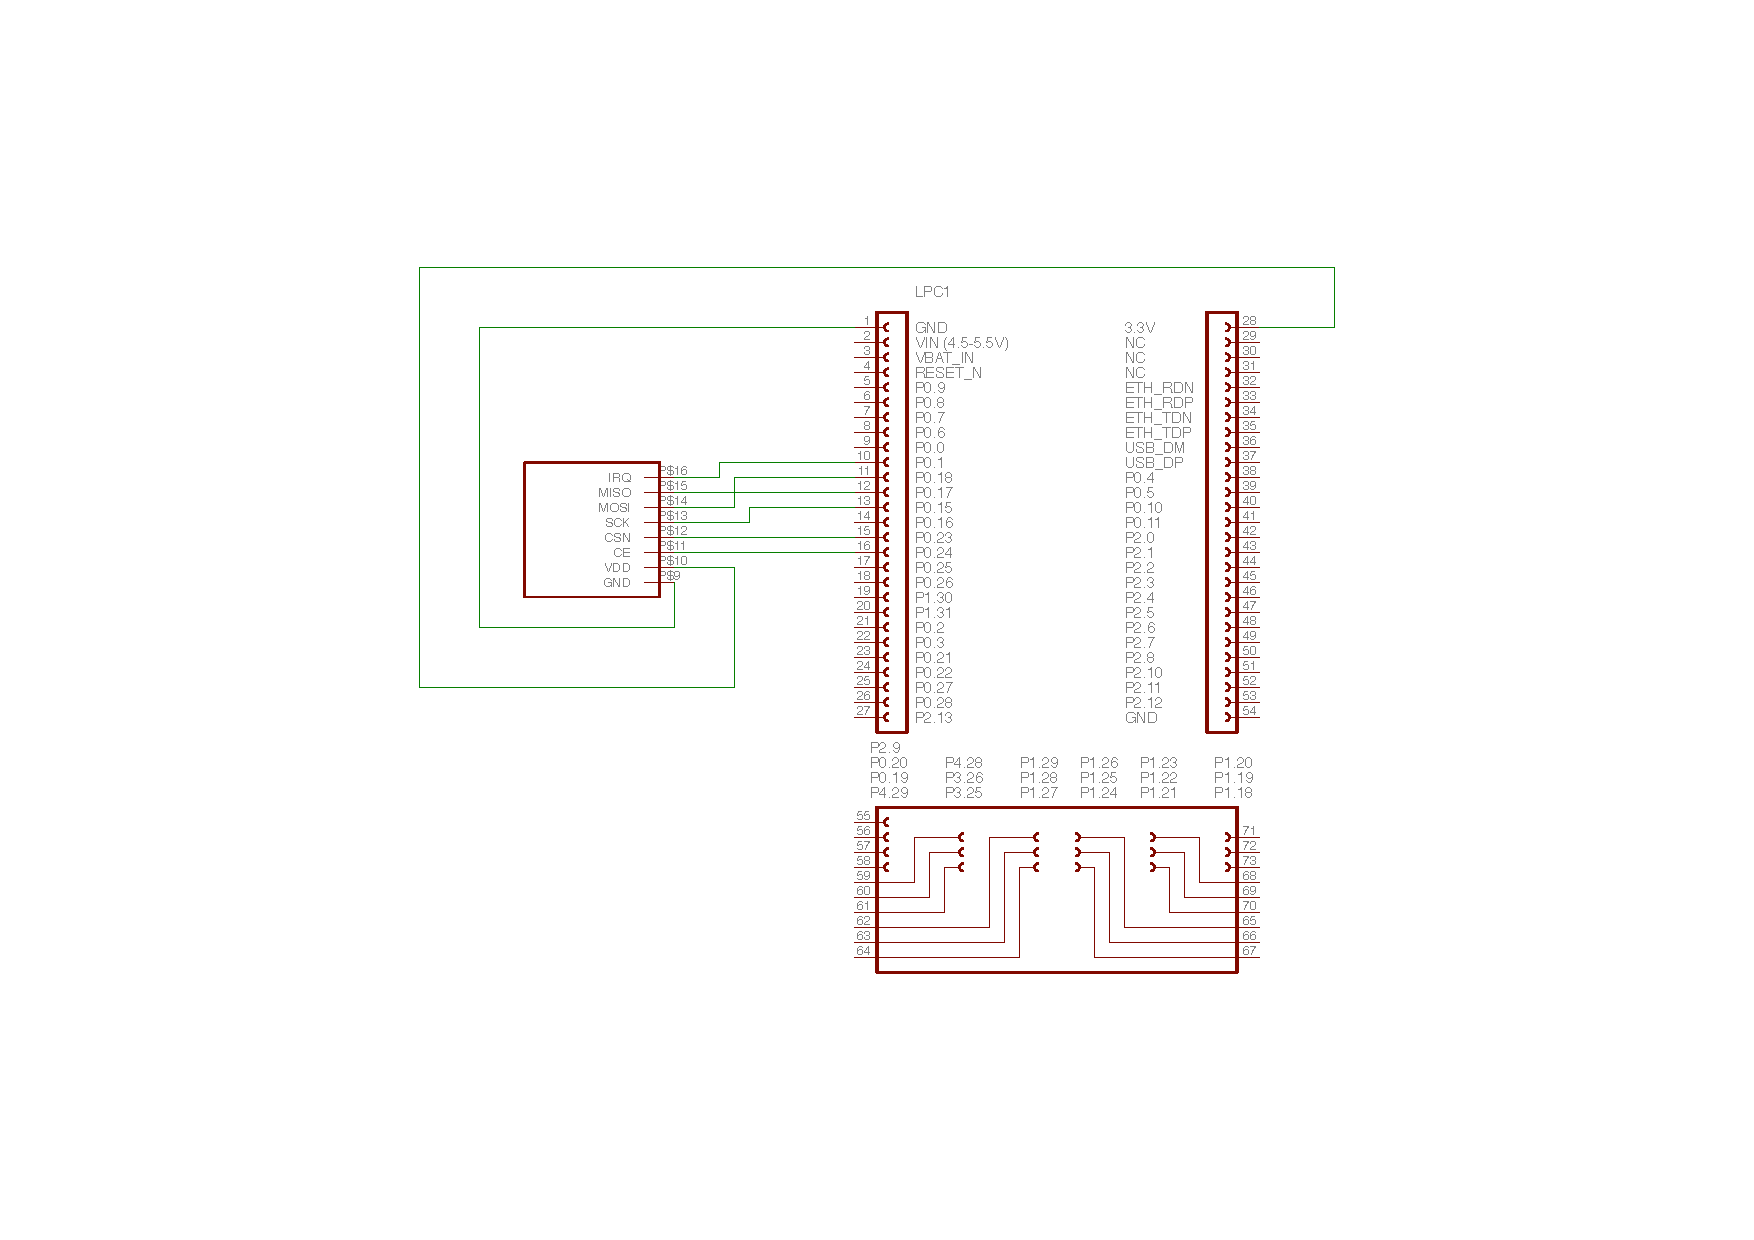
\includegraphics[scale=1, clip, trim=0 40mm 0 40mm]{example_rfm}}
\caption{Schemat podłączenia modułu RFM73 do płytki prototypowej z mikrokontrolerem LPC1769}
\label{fig:examplerfm}
\end{figure}


\subsection{Uzyskane wyniki}

Implementowany sterownik miał zapewnić abstrakcję modułu RFM73 z poziomu aplikacji napisanej w~języku Erlang z interfejsem pozwalającym na łatwe wysyłanie i odbieranie wiadomości drogą radiową. W celu przetestowania działania modułu, wysłano zestaw krótkich pakietów do innego urządzenia z podłączonym modułem tego samego typu. Program odbierający wiadomości po drugiej stronie odpowiadał wiadomościami o tej samej treści, dzięki czemu zweryfikowano poprawność danych przesyłanych w~dwie strony.


\subsection{Wnioski}

Zaimplementowana biblioteka może być również podstawą do implementacji protokołu \emph{Distributed Erlang}, dzięki któremu możliwy byłby do uruchomienia klaster urządzeń komunikujących się za pomocą modułu RFM73.